% Propósito: relacionar el recorrido adicional de una reflexión con su retardo
% y evitar interpretar ese retardo como un umbral perceptual universal.
% Origen: Delta t=Delta r/c, ecuación
% \eqref{eq:u7-retardo-reflexion}, y discusión de la sección
% \ref{sec:u7-precedencia}. Geometría esquemática sin escala.
% Descripción accesible: el panel izquierdo muestra una fuente, un oyente y una
% pared; una flecha recta representa la llegada directa y otra, más larga,
% rebota en la pared. El panel derecho muestra dos llegadas sobre un eje
% temporal separadas por Delta t. Una nota indica que la percepción depende de
% otras propiedades además del retardo.
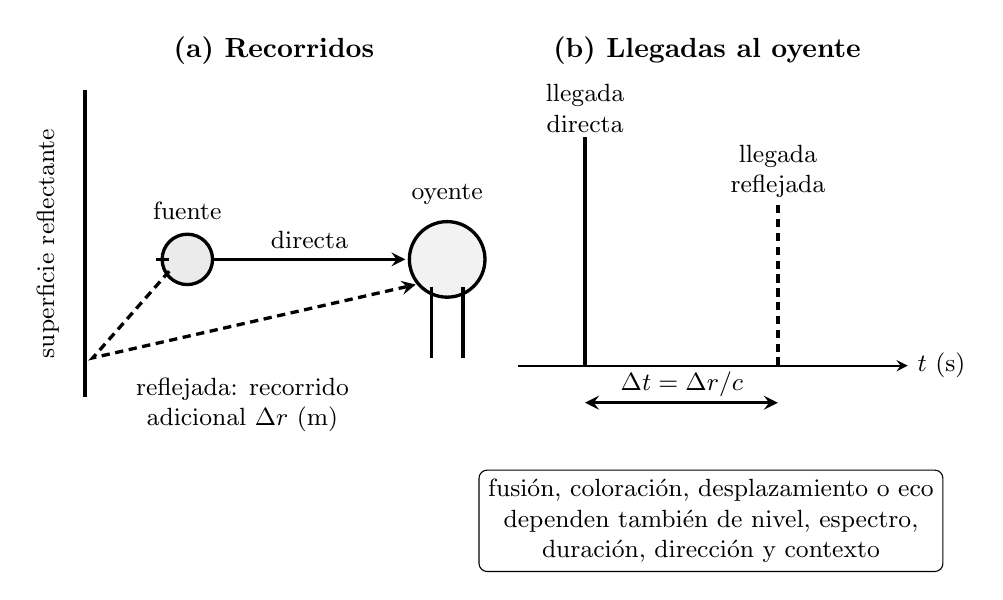
\begin{tikzpicture}[font=\small,>=stealth,x=1cm,y=1cm]
    \node[font=\bfseries] at (3.15,5.25)
        {(a) Recorridos};
    \draw[very thick] (0.75,0.85) -- (0.75,4.75);
    \node[rotate=90] at (0.28,2.80) {superficie reflectante};

    \draw[very thick,fill=black!8] (2.05,2.60) circle (0.32);
    \draw[very thick] (1.65,2.60) -- (1.82,2.60);
    \node[anchor=south] at (2.05,2.98) {fuente};

    \draw[very thick,fill=black!5] (5.35,2.60) circle (0.48);
    \draw[very thick] (5.15,2.25) -- (5.15,1.35);
    \draw[very thick] (5.55,2.25) -- (5.55,1.35);
    \node[anchor=south] at (5.35,3.18) {oyente};

    \draw[->,very thick] (2.38,2.60) -- (4.82,2.60)
        node[midway,above] {directa};
    \draw[->,very thick,densely dashed]
        (1.82,2.45) -- (0.85,1.35) -- (4.95,2.28);
    \node[align=center] at (2.75,0.75)
        {reflejada: recorrido\\adicional \(\Delta r\) (m)};

    \node[font=\bfseries] at (8.65,5.25)
        {(b) Llegadas al oyente};
    \draw[->,thick] (6.25,1.25) -- (11.20,1.25);
    \node[anchor=west] at (11.20,1.25) {\(t\) (s)};
    \draw[very thick] (7.10,1.25) -- (7.10,4.15);
    \draw[very thick,densely dashed] (9.55,1.25) -- (9.55,3.35);
    \node[align=center] at (7.10,4.52) {llegada\\directa};
    \node[align=center] at (9.55,3.72) {llegada\\reflejada};
    \draw[<->,very thick] (7.10,0.78) -- (9.55,0.78);
    \node[fill=white,inner sep=1.5pt] at (8.33,1.02)
        {\(\Delta t=\Delta r/c\)};

    \node[draw,rounded corners=3pt,align=center,fill=white,
        minimum width=4.50cm] at (8.70,-0.72)
        {fusión, coloración, desplazamiento o eco\\
         dependen también de nivel, espectro,\\
         duración, dirección y contexto};
\end{tikzpicture}
